
The United States have been the forerunner of nuclear energy, with a currently 
installed nuclear capacity of 100,350 \gls{MWe} \cite{iaea_nuclear_2017}.
With its size and long history of nuclear
energy, the United States have accumulated about $70,000$ \gls{MTHM} of \gls{UNF}.

The problem with modeling the U.S. transition scenario is that the U.S. does not have
a defined advanced reactor, whereas France has a central plan to transition into \glspl{ASTRID} \cite{boullis_french_2015, varaine_pre-conceptual_2012}.
Previous analyses \cite{worrall_utilization_2013, sunny_transition_2015} focused on transitioning into
fast-spectrum \glspl{SFR}.
However, the fact that the U.S. nuclear reactor fleet
is decided by economic interests (industries), this leads to
a need to explore different options, such as transitioning into \glspl{MSR}.

As explained in section \ref{sec:msr}, rising interests in \gls{MSR} designs
led to a proliferation of U.S. corporations aiming to commercialize
\gls{MSR} designs. Given the large interest from industries,
\gls{MSR} reactor designs are
most likely to be commercially deployed in the United States.

In this chapter, I explore the U.S. transition scenario
from a \gls{LWR} fleet into a \gls{MSR} fleet.

\section{Initial Conditions and Scenario Parameters}

For the French scenario, the \gls{UNF} inventory at the present
time is calculated by simulating the nuclear operational history from 1970.
However, this is unnecessary for the U.S. scenario because there is a 
detailed database that describes the U.S. \gls{UNF} inventory up to May of 2013.
The \gls{UNF-STANDARDS} is a comprehensive,
controlled source of \gls{UNF} information, including dry cask attributes, assembly
data, and economic attributes \cite{peterson_unf-st&dards_2017}. This database
allows the transition scenario simulation to start from 2013, instead of 1970,
as in the French simulation. The \gls{UNF} inventory mass and composition in 2013
is imported from \gls{UNF-STANDARDS} and is `initiated' in the simulation
as a \texttt{Source} facility. The total mass of \gls{UNF} listed
in the \gls{UNF-STANDARDS} database is 68,072 MTHM.

Furthermore U.S. currently has additional uranium resource in the
form of more than $700,000$ MTHM of depleted uranium \cite{office_nuclear_2011},
which is a waste product of enrichment. The depleted uranium inventory
is currently a liability and waste, but can be utilized as fertile material
in a U-Pu fuel cycle. If the U.S. chooses a Th-$^233U$ fuel cycle,
additional thorium resources would be needed, while with a U-Pu cycle, the
U.S. can use its waste to create fuel.

The U.S. nuclear fleet in 2013 can be extracted from the \gls{PRIS} database.
The same assumption that legacy reactors have a 60-year lifetime is applied.
I used \texttt{write\_input.py} to generate the expected power capacity
of the current U.S. nuclear from 2013 (shown in figure \ref{fig:us_legacy}).

\begin{figure}[htbp!]
	\begin{center}
		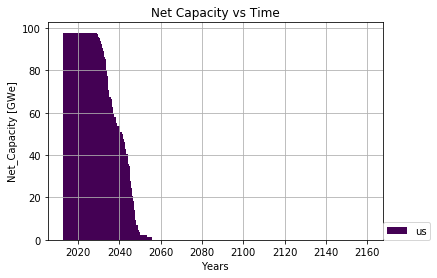
\includegraphics[scale=0.6]{./images/us/legacy_power.png}
	\end{center}
	\caption{Installed nuclear capacity in the United States from 2013.}
	\label{fig:us_legacy}
\end{figure}

The U.S. had 101 reactor units operating in 2013. Two reactors -
Vermont Yankee and Fort Calhoun One - has shut down since 2013.
Vermont Yankee was shut down in December, 2014, and Fort
Calhoun One was shut down in October, 2016. At the date of this
work, the United States has 99 commercial reactors with a 
net capacity of 100,350 \gls{MWe} \cite{iaea_nuclear_2017}.


\subsection{Energy Demand Prediction}
The reference for the energy demand prediction is the 
\gls{EIA} Annual Energy Outlook \cite{u.s._eia_annual_2018}.
The 2018 Annual Energy Outlook report predicts an annual electricity demand growth
of 0.9\%. The report also predicts that nuclear
power will either remain static or decrease. The report
predicts that nuclear capacity will decrease from 99 GWe
to 79GWe in 2050, with no new plants beyond 2020.
However, for this work,
I assume that the U.S. nuclear power capacity is kept at the
current capacity, and new reactors are deployed to make up for the
decommissioned capacity.

\subsection{\gls{MSR} Design and Availability}

\gls{MSR} designs can be categorized depending on their operating
neutron spectrum (e.g. fast, thermal), fuel cycle (e.g. Th-$^{233}U$, U-Pu),
and transmutation goals (e.g. breeder, burner). Selection of an \gls{MSR}
design depends on various factors like economics, safety, and fuel cycle
considerations. For this work, I choose a fast, U-Pu cycle, burner \gls{MSR} design
named REBUS-3700 \cite{mourogov_potentialities_2006} to deploy for the
transition analysis.

The REBUS-3700 \gls{MSR} design offers four principal
advantages over other \gls{MSR} designs:
\begin{itemize}
	\item Fast spectrum - no need for moderator rods 
	\item U-Pu cycle - requires only depleted uranium for supply after initial fuel salt loading
	\item Weakly positive breeding gain (0.03)
	\begin{itemize}
		\item Self-sufficient (no external fissile input)
		\item No surplus fissile material production (stabilizes Pu inventory)
	\end{itemize}
	\item U-\gls{TRU} initial fuel - transmutation of long-lived actinides
	\item Simpler design - no radial / axial blanket
\end{itemize}

The U.S. has a large inventory of \gls{LWR} \gls{UNF} and tails. The benefits
of the REBUS-3700 design aligns with the waste management interest
of the U.S of reducing final geological repository burden. The U.S. can dramatically reduce its repository
burden by:

\begin{itemize}
	\item Reduction of \gls{TRU} inventory by transmutation in the reactor (table \ref{tab:rebus_comp})
	\begin{itemize}
		\item Reduction of long-term decay heat and activity (figure \ref{fig:decay_heat})
		\item More `tailored' waste form design for fission products
	\end{itemize}
	\item Reducing tails inventory
\end{itemize}

Additionally, the REBUS-3700 does not have, at any moment in
operation, separated fissile streams, like other \gls{MSR} designs
such as the \gls{MSBR} design \cite{robertson_conceptual_1971} (protactinium tank for
$^{233}U$),
or the \gls{MCSFR} design \cite{smith_assessment_1974} (separated Pu stream from the blanket region).
The REBUS-3700 only takes in depleted uranium and processes out
fission product groups such as volatile gases and noble metals.
The detailed reprocessing scheme is shown
in table \ref{tab:rebus_reproc}. 
This self-sustained and closed operation increases its non-proliferation
properties.

The REBUS-3700 initial fuel and equilibrium \gls{TRU} isotopic composition is
shown in table \ref{tab:rebus_comp}. The \gls{TRU} isotopic composition
matches that of the \gls{LWR} \gls{UNF} after 8.5 years of decay (shown
in figure \ref{fig:trutru}). 


\begin{figure}[htbp!]
	\begin{center}
		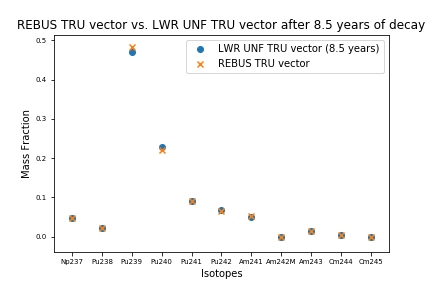
\includegraphics[scale=0.6]{./images/us/trutru.png}
	\end{center}
	\caption{\gls{TRU} vector of REBUS-3700 initial fuel from Mourogov et al. \cite{mourogov_potentialities_2006}
		with \gls{LWR} \gls{UNF} after 8.5 years of decay}
	\label{fig:trutru}
\end{figure}


\begin{table}[h]
	\centering
	\caption{Initial and equilibrium \gls{TRU} isotopic composition from literature \cite{mourogov_potentialities_2006}.}
	\label{tab:rebus_comp}
	\begin{tabular}{lll}
		\hline
		Isotope & Beginning of Life & Equilibrium (\textasciitilde 6500 \gls{EFPD}) \\
		\hline
		$^{237} Np$ / $^{239} Np$ &  4.80 / 0.00 & 0.65 / 0.07 \\
		$^{238} Pu$ / $^{239} Pu$ / $^{240} Pu$ / $^{241} Pu$ / $^{242} Pu$ & 2.13 / 48.33 / 22.17 / 9.05 / 6.38 & 2.23 / 58.02 / 27.63 / 3.35 / 4.05 \\
		$^{241} Am$ / $^{242m} Am$ / $^{243} Am$ &5.17 / 0.01 / 1.48 & 1.50 / 0.12 / 1.05 \\
		$^{242} Cm$ / $^{243} Cm$ / $^{244} Cm$ / $^{245} Cm$ / $^{246} Cm$ & 0.0 /0.0 / 0.43 / 0.04 / 0.00 & 0.07 / 0.01 / 1.02 / 0.19 / 0.05 \\
		Equivalent enrichment, \% & 10.1 & 11.0 \\
		\gls{TRU} fraction in heavy atoms vector, \% & 15.6 & 15.9 \\
		\hline
	\end{tabular}
\end{table}

I performed a preliminary feasibility study of the two initial fuel compositions using Saltproc.
Results (in figure \ref{fig:rebus_diff}) show that the core with \gls{LWR} \gls{UNF} \gls{TRU}
composition has a higher $k_{eff}$ value in the beginning, but shows little difference after
the first ten years. A lifetime of 40 years for the REBUS-3700 reactor is set since the $k_{eff}$
value drops below 1.01 after 40 years of operation. The \gls{TRU} composition for the end-of-life
fuel salt is shown in table \ref{tab:eol_comp}.


\begin{table}[h]
	\centering
	\caption{Beginning-of-life and end-of-life \gls{TRU} composition in the REBUS-3700 design with modified initial fuel composition.}
	\label{tab:eol_comp}
	\begin{tabular}{lll}
		\hline
		Isotope & Beginning of Life & End of Life \\ 
		\hline
		Np237 & 4.80E-02 & 8.24E-03\\ 
		Np239 & 0.00E+00 & 5.49E-04\\ 
		Pu238 & 2.13E-02 & 2.72E-02\\ 
		Pu239 & 4.84E-01 & 5.53E-01\\ 
		Pu240 & 2.22E-01 & 2.84E-01\\ 
		Pu241 & 9.05E-02 & 3.29E-02\\ 
		Pu242 & 6.38E-02 & 4.56E-02\\ 
		Am241 & 5.17E-02 & 1.87E-02\\ 
		Am243 & 1.48E-02 & 1.39E-02\\ 
		Cm242 & 0.00E+00 & 7.62E-04\\ 
		Cm244 & 4.30E-03 & 1.11E-02\\ 
		Cm245 & 4.00E-05 & 2.76E-03\\ 
		Cm246 & 0.00E+00 & 9.63E-04\\ 
		Cm247 & 0.00E+00 & 1.23E-04\\ 
		\hline
	\end{tabular}
\end{table}


\begin{table}[h]
	\centering
	\caption{Reprocessing scheme for REBUS-3700}
	\label{tab:rebus_reproc}
	\begin{tabular}{lll}
		\hline
		Group & Elements & Reprocessing Time (s) \\
		\hline    
		Volatile Gases & Kr, Xe, Ar, Ne, H, N, O, Rn & 30 \\
		Noble Metals & \shortstack{Se, Nb, Mo, Tc, Ru, Rh,\\ Pd, Ag, Sb, Te, Zr, Cd, In, Sn} & 30 \\
		Rare Earths & \shortstack{Y, La, Ce, Pr, Nd, Pm, Sm, Gd, \\ Eu, Dy, Ho, Er, Tb, Ga, Ge, As, Zn} & 259200 \\
		\hline
	\end{tabular}
\end{table}



\section{U.S. Deployment Schedule}

As shown in figure \ref{fig:us_legacy}, the U.S. will
undergo a large loss of nuclear capacity from 2030, under the
assumption that U.S. reactors have a lifetime of 60 years.

Since it is unlikely that \glspl{MSR} are ready for
commercial deployment in 2020, I deploy \glspl{LWR} (AP 1000 design \cite{sutharshan_ap1000tm_2011})
to make up for the decommissioned capacity. After 2050,
REBUS-3700 design \glspl{MSR} are deployed. The deployment of new reactors
are shown in figure \ref{fig:us_dep}, and the installed
power capacity of the reactors is shown in \ref{fig:us_pow}.
In the simulation, 84 additional \glspl{LWR} and 95 \glspl{MSR}
are deployed.

\begin{figure}[htbp!]
	\begin{center}
		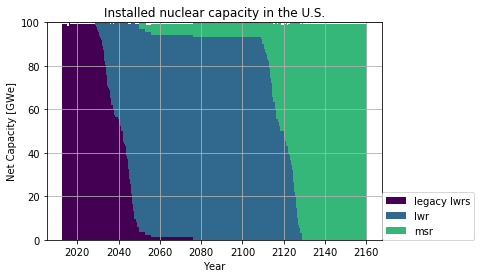
\includegraphics[scale=0.6]{./images/us/power_plot.png}
	\end{center}
	\caption{New reactor deployment from 2020.}
	\label{fig:us_pow}
\end{figure}

\begin{figure}[htbp!]
	\begin{center}
		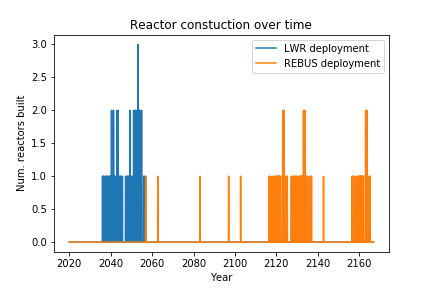
\includegraphics[scale=0.6]{./images/us/us_dep.png}
	\end{center}
	\caption{New reactor deployment from 2020.}
	\label{fig:us_dep}
\end{figure}

\section{Material Flow}

The fuel cycle is represented by a series of facility agents whose material 
flow is illustrated in figure \ref{diag:us_fc}, along with
the \Cyclus archetypes that were used to model each facility.

\begin{figure}
	\centering
	\scalebox{0.6}{
		\begin{tikzpicture}[align=center, node distance = 3cm and 3cm, auto]
		% Place nodes
		\node [block] (sr) {Mine (\texttt{SOURCE})};
		\node [cloud, below of=sr] (nu) {Nat U};
		\node [block, below of=nu] (enr) {Enrichment ({\footnotesize \texttt{ENRICHMENT}})};
		\node [cloud, below of=enr] (uox) {\acrshort{UOX}};
		\node [block, below of=uox] (lwr) {\gls{LWR} (\texttt{REACTOR})};
		\node [cloud, right of=lwr] (snf) {\gls{UNF}};
		\node [block, right of=snf] (pool) {Pool (\texttt{Storage})};
		\node [cloud, left of=uox] (tl2) {Dep U};
		\node [block, below of=tl2] (stor) {Storage (\texttt{Storage})};
		\node [block, right of=tl] (sk) {Repository (\texttt{SINK})};
		\node [cloud, below of=sk] (cunf) {Cooled \gls{UNF}};
		\node [cloud, below of=pool] (cunf2) {Cooled \gls{UNF}};
		\node [block, below of=snf] (rep) {{\small Reprocessing ({\footnotesize \texttt{SEPARATIONS}})}};
		\node [cloud, below of=rep] (u) {Sep. U} ;
		\node [cloud, left of=rep] (pu) {Sep. TRU};
		\node [block, left of=pu] (mix) {Fabrication (\texttt{MIXER})};
		\node [cloud, below of=mix] (fs) {Fuel Salt};
		\node [block, below of=mox] (mxr) {\gls{MSR} (\texttt{HDF5-Reactor})};
		\node [cloud, left of=stor] (tl) {Dep U};
		
		\node [cloud, right of=mxr] (waste) {Waste};
		\node [cloud, right of=fs] (es) {End-of-life Salt};
		
		\draw[->, thick] (sr) -- (nu);
		\draw[->, thick] (nu) -- (enr);
		\draw[->, thick] (enr) -- (tl2);
		\draw[->, thick] (tl2) -- (stor);
		\draw[->, thick] (enr) -- (uox);
		\draw[->, thick] (uox) -- (lwr);
		\draw[->, thick] (lwr) -- (snf);
		
		\draw[->, thick] (lwr) -- (snf);
		\draw[->, thick] (snf) -- (pool);
		\draw[->, thick] (pool) -- (cunf);
		\draw[->, thick] (pool) -- (cunf2);
		\draw[->, thick] (cunf) -- (sk);
		\draw[->, thick] (cunf2) -- (rep);
		
		\draw[->, thick] (rep) -- (u);
		\draw[->, thick] (rep) -- (pu);
		\draw[->, thick] (pu) -- (mix);
		\draw[->, thick] (mix) -- (mox);
		\draw[->, thick] (mox) -- (mxr);
		
		\draw[->, thick] (stor) -- (tl);
		\draw[->, thick] (tl) to [bend right] (mxr);
		\draw[->, thick] (tl) -- (mix);
		\draw[->, thick] (nu) -- node{} ++ (-8cm, 0) |- (mix) ;
			
		\draw[->, thick] (mxr) -- (waste);
		\draw[->, thick] (waste) to [bend right=80] (sk);
		\draw[->, thick] (mxr) -- (es);
		\draw[->, thick] (es) -- (rep);
		
		\end{tikzpicture}
		
	}
	\caption{Fuel cycle facilities (blue boxes) represented by 
		\Cyclus archetypes (in parentheses) pass materials (red 
		ovals) around the simulation.} 
	\label{diag:us_fc}
\end{figure}

The U.S. transition scenario's material flow is similar to that of France,
except that all \gls{TRU} is reprocessed from \gls{LWR} \gls{UNF}
to fabricate fuel salt. Also, the depleted uranium from
the enrichment plant is stored in a storage facility to be used as a fertile stream for \gls{MSR} facilities.
Natural uranium is mixed with the reprocessed \gls{TRU} to create fuel salt.
Lastly, instead of a single
stream of \gls{MOX} \gls{UNF} from the \gls{MOX} reactors, the \gls{MSR}
outputs two streams - waste and end-of-life salt - that is disposed
and reprocessed, respectively.

\FloatBarrier


\section{Scenario Specification}

The scenario specifications defining the simulations presented in this chapter
are listed in table \ref{tab:us_sim_specs}.

\begin{table}[h]
	\centering
	\caption{Simulation Specifications}
	\begin{tabularx}{\linewidth}{bss}
		\hline
		\textbf{Specification} &\textbf{ Value} & \textbf{Units}\\
		\hline
		Simulation Starts & 2013 & year\\
		Simulation Ends & 2160 & year\\ 
		Production of \gls{MSR} fuel begins & 2030 & year\\
		\glspl{MSR} become available & 2050 & year\\
		Reprocessed uranium usage &  None & -\\
		Minimum \gls{UNF} cooling time  & 8.5  & years\\
		Separation efficiency of U and Pu & 99.8 & \% \\
		Reprocessing streams & \gls{TRU} and U & - \\
		Reprocessing capacity & $\infty$ & $\frac{\text{metric tons of \gls{UNF}}}{month}$\\
		\gls{MSR} fuel salt fabrication throughput & No limit ($\infty$) & $\frac{\text{metric tons}}{month}$ \\
		\gls{MSR} fuel salt recycling & $\infty$-pass & - \\
		\hline
	\end{tabularx}
	\label{tab:us_sim_specs}
\end{table}

\section{Reactor Specifications}

Two major reactors are used in the simulation, \gls{PWR} and \gls{MSR}
reactors. 

For \glspl{PWR}, I use a linear core size model to capture varying reactor capacity
(explained in section \ref{sec:writeinput}). The reactors deployed after 2020 are
modeled after the AP-1000 reactor \cite{sutharshan_ap1000tm_2011}. The reactor
specifications are shown in \ref{tab:us-reactor-specs}.

\begin{table}[h]
	\centering
	\caption{Baseline \gls{LWR} and \gls{MSR} simulation specifications.}
	\begin{tabular}{lrr}
		\hline
		\textbf{Specification} & \textbf{\gls{PWR} \cite{sutharshan_ap1000tm_2011}} & \textbf{\gls{MSR} \cite{mourogov_potentialities_2006}} \\
		\hline
		Lifetime [y]  & 80 & 40 \\
		Cycle Time [mos.]& 18 & continuous \\ 
		Refueling Outage [mos.]& 2 & N/A \\
		Rated Power [\gls{MWe}] & 1110 & 1628 \\
		Assembly mass [kg] & 446 & N/A \\
		Batch mass [kg] & 23,192 & N/A \\
		Core mass [kg] & 70,022 & 200,100 \\
		Discharge Burnup [GWd/tHM] & 51 & N/A \\
		Assemblies per core & 157  & N/A \\
		Batches per core & 3 & N/A \\
		Initial Fissile Loading [t] & 3.1  $^{235}$U & 18.06 \gls{TRU} \\
		Fuel & \gls{UOX} & \gls{TRU}-U Cl Salt \\
		\hline
	\end{tabular}
	
	\label{tab:us-reactor-specs}
	
\end{table}


\section{Material Definitions}
Depletion calculations for the \gls{LWR} nuclear fuel are recipe-based, such 
that a fresh and used fuel recipe is calculated beforehand using ORIGEN (see table \ref{tab:comp}).
ORIGEN calculates buildup, decay and processing of radioactive materials
\cite{parks_overview_1992}. This recipe has also been used for
repository performance modeling \cite{wilson_adoption_2009}.
For fresh \gls{LWR} fuel, I assume a fuel enrichment of 3.1\% U235.

For depletion calculations for \gls{MSR} fuel, I use Saltproc (section \ref{sec:saltproc})
to obtain depleted fuel compositions and waste stream composition in a continuously
reprocessing reactor operation.

\section{Database Generation}
The HDF5 database for this simulation is generated using Saltproc
and a unit cell model of the REBUS-3700 reactor. The parameters
used for running SERPENT and Saltproc are shown in table \ref{tab:saltproc-run-params}.

\begin{table}[h]
	\centering
	\caption{Saltproc simulation parameters used to generate the database for REBUS-3700}
	\begin{tabular}{lr}
		\hline
		\textbf{Parameter} & \textbf{Value}\\
		\hline
		\multicolumn{2}{c}{\textbf{SERPENT Parameters}} \\
		\hline
		Num. neutrons per generation & 8,000 \\
		Num. active generation & 150\\
		Num. inactive generation & 50 \\
		Burnup calc. mode & CRAM \\
		Power density & $32.18e-3$ $\frac{kW}{g}$ \\ 
		Depletion step & 30 days\\
		Fuel salt density & $3.6 \frac{g}{cm^3}$ \\		
		\hline
		\multicolumn{2}{c}{\textbf{Saltproc Parameters}} \\
		\hline
		Lifetime [y]  & 60 \\
		Total timesteps & 365 \\
		Reprocessing Scheme & As table \ref{tab:rebus_reproc}\\
		Refill material & Depleted uranium ($0.3\%$ $^{235}U$) \\
		\hline
	\end{tabular}
	
	\label{tab:saltproc-run-params}
	
\end{table}
\section{Results}

\section{Conclusion}